\documentclass[12pt,letterpaper]{article}
\usepackage[margin=1.25in]{geometry}
\usepackage{authblk}
\usepackage{graphicx}
\usepackage{booktabs}
\usepackage{tabularray}
\usepackage{float}
\usepackage[normalem]{ulem}
\UseTblrLibrary{booktabs}
\UseTblrLibrary{siunitx}
% ASA style omits leading zeros (e.g., .06 instead of 0.06); siunitx
% otherwise reinserts them by default.
\sisetup{print-zero-integer=false}
\newcommand{\tinytableTabularrayUnderline}[1]{\underline{#1}}
\newcommand{\tinytableTabularrayStrikeout}[1]{\sout{#1}}
\NewTableCommand{\tinytableDefineColor}[3]{\definecolor{#1}{#2}{#3}}
\usepackage{hyperref}
\hypersetup{
  colorlinks=true,
  linkcolor={blue},
  filecolor={magenta},
  citecolor={blue},
  urlcolor={blue}
}\usepackage{setspace}
\usepackage{natbib} 
\bibliographystyle{apalike} 


\doublespacing

\title{Patriotism as a Choice Process: National Pride After 9/11\thanks{Direct correspondence to Omar Lizardo, [INSERT DEPARTMENT], University of California, Los Angeles, [INSERT MAILING ADDRESS] (\href{mailto:REPLACE@ADDRESS.EDU}{REPLACE@ADDRESS.EDU}). [INSERT ACKNOWLEDGMENTS, e.g., prior presentations of this work or colleagues thanked for comments.] [INSERT GRANT/FUNDING INFORMATION, or state: ``This research received no specific grant from any funding agency.'']}}
\author{Omar Lizardo}
\affil{UCLA}
\date{\today}

\begin{document}
\maketitle

\begin{center}
\textit{Running Head: [INSERT RUNNING HEAD, 60 CHARACTERS OR FEWER]}\\
\textit{Word Count: Approximately 6,300 words (main text, abstract, and notes; excludes tables, figures, and reference list)}
\end{center}

\newpage
\section*{Biography}
[INSERT AUTHOR BIOGRAPHY, 100 WORDS OR FEWER -- name, title, department, institution, and a brief description of current research interests, publications, or awards. E.g.: Omar Lizardo is [TITLE, e.g., Professor of Sociology] in the Department of Sociology at the University of California, Los Angeles. His research interests include [RESEARCH INTERESTS]. His recent work has appeared in [PUBLICATIONS/AWARDS].]

\newpage
\begin{abstract}
Which groups are more likely to experience increased feelings of national pride after experiencing a threat to the nation? Using survey data on a representative sample of Americans collected before and during the post-9/11 period in the United States---with the September 11 attacks serving as the catalyzing event for a broader climate of national mobilization that included the onset of the wars in Afghanistan and Iraq---this paper adjudicates between competing hypotheses regarding the socio-demographic distribution of national pride. Theories of ``irrational patriotism'' and needs-based attachments predict that lower-status individuals will experience the largest increase in national pride. In contrast, the choice-process approach suggests that higher-status individuals---who experience greater autonomy and are more likely to be embedded in nested voluntary associations---will be more likely to increase their affective attachment to the national collectivity under a ``distal'' attribution rule. Results from the General Social Survey (1996 and 2004) support the choice-process theory, demonstrating that educated individuals and members of specific nested subgroups experienced the most significant increases in national pride post-9/11.
\end{abstract}

\vspace{1em}
\noindent\textbf{Keywords:} [KEYWORD 1], [KEYWORD 2], [KEYWORD 3], [KEYWORD 4], [KEYWORD 5]

\newpage
\section{Introduction}

Which groups are more likely to experience increased feelings of national pride after experiencing a threat to the nation? In this paper, I use survey data on a representative sample of Americans collected before and during the post-9/11 period to shed light on this question. I treat the September 11 attacks not as an isolated, punctual stimulus but as the catalyzing event that opened a broader period of sustained national mobilization---one that also encompassed the U.S. invasion of Afghanistan and the buildup to the Iraq War---and it is this period, rather than 9/11 as a single dated event, that constitutes the theoretical object of interest. This ``natural experiment'' allows me to adjudicate between competing hypotheses regarding the socio-demographic distribution of feelings of national pride following a threat to the nation.

Theories in the tradition of the ``authoritarian personality'' \citep{adorno1950authoritarian-a52} and the modern political science of the personality correlates of political ideology \citep{jost2007are-871, jost2017ideology-f69, jost2008ideology-368} conceive of national pride as reflecting a form of ``irrational patriotism,'' driven by fundamentally ingrained motivational and affective factors that differ across people. These theories predict that members of low-status groups will be much more likely to experience renewed feelings of national pride after experiencing a threat to the nation. From this perspective, a threat to the nation is seen as endangering the ``ontological security'' \citep{giddens1984constitution} of persons whose lives are characterized by routine and alienating work, who are disengaged from established institutions, or who have been left behind by recent structural changes to the economy and rapid cultural shifts in dominant values \citep{wuthnow2019left-c34}.

Theories of attachment to collectivities as a nested group \citep{lawler1992affective-8c8, mueller1999commitment}, on the other hand, point to a different dynamic and lead to a clearly divergent empirical implication. According to the choice-process approach, individuals are more likely to experience affective attachment to a larger group within which other groups that they belong to are nested (such as the nation), \textit{only} to the extent that they are able to in fact experience freedom and autonomy in their everyday dealings, and to the extent that this autonomy and freedom is \textit{attributed} to membership both in the more proximate groups that they are part of, and to the larger unit within which these groups are nested. 

These two propositions suggest that, given that high status individuals are more likely to be in structural positions that afford autonomy and self-direction \citep{kohn1969class, kohn1977class-ee1, kohn1978reciprocal-f1b}, and given that they are more likely to belong to ``nested-subgroups," such as voluntary associations \citep{bell1956social, freeman1957correlates, janoski1996pathways, knoke1986associations, mcpherson1981dynamic, scott1957membership, tomeh1973formal, dederichs2024join-411}, within which feelings of attachment to super-ordinate collectivities can be fostered and made salient, the choice-process theory predicts that it will be high-status individuals who will be more likely to experience renewed feelings of national pride following a threat to the nation.

In this paper, I adjudicate between these two competing predictions by drawing on nationally representative survey data collected shortly before and shortly after the events of September 11, 2001. I first review the theoretical logic underlying the irrational patriotism and choice-process approaches in greater detail, deriving testable hypotheses regarding the expected socio-demographic distribution of national pride and nationalism following a threat to the nation. I then describe the data, measures, and modeling strategy used to test these hypotheses, before presenting results bearing on the period shift in national pride, the role of education as a proxy for structural autonomy, and the role of nested voluntary association memberships in fostering affective attachment to the nation. I conclude by discussing the implications of these findings for theories of national attachment and outlining directions for future research.

\section{Where Does National Pride Come From? Two Approaches}

\subsection{The Needs-Based and irrational patriotism Models}

Standard approaches in social psychology geared toward explaining individual differences in affective attachment to nations as collectivities usually point to factors associated with the emotional needs that such feelings of national pride meet \citep{jost2007are-871}. Thus, classic studies of the authoritarian personality noted how persons who scored high on authoritarianism scales were also prone to express ``irrational'' feelings of pride and ``blind'' attachment to the nation conceived as a solidary collectivity \citep{adorno1950authoritarian-a52, pettigrew1999placing}. Excessive attachment to national groups is usually regarded as pathological and as leading to various suboptimal societal outcomes, such as support for authoritarian or charismatic leaders and less support for democratic or inclusive institutions \citep{santos2024liberal-conservative-a61}.\footnote{Social Identity Theory and Self-Categorization Theory can also be considered ``need-based'' theories \citep{hogg2000social-e0d}. In these frameworks, the self-enhancement motive leads individuals to become affectively attached to prestigious national collectivities. Individuals become attached to national groups in the very same way that they become attached to any other group---if the group is perceived as meeting emotional needs for self-esteem, prestige, and a sense of efficacy and belonging. } 

If feelings of national pride are an expression of either authoritarianism or irrational patriotism, then we should find it overrepresented among those groups marked by the socio-demographic characteristics typically associated with these cognitive and affective orientations. The bulk of the research suggests this refers to low-status, low-education groups, typically alienated from mainstream institutions and disempowered in their everyday interactions \citep{collins1986weberian, jost2017working-608, jost2003social-206}. This implies that post-9/11 increases in national affective attachment in the U.S. should be concentrated among lower-status groups, who may be more likely to react to epistemic and existential threats to the status quo by becoming affectively attached to the nation, thereby increasing their belief in the propriety and desirability of existing systems.

\subsection{Lawler's Choice-Process Theory and Nested Attachments}

In contrast to needs-based and irrational patriotism views, Edward Lawler's \citeyearpar{lawler1992affective-8c8} choice-process theory posits a different mechanism. According to the theory, people value individuality, freedom, and self-efficacy, and they engage in structured action within concrete social contexts, primarily nested subgroups, to enact those values. In this way, groups provide individuals with a ``context of choice'' within which successful purposive action occurs. Positive emotions stemming from the sense of autonomy and control afforded by the group trigger an attribution process that leads people to become affectively attached to those groups and, by implication, to any larger group within which those groups are nested.

From this perspective, national ``groups''--closer to ``imagined communities'' in Anderson's \citeyearpar{anderson1991imagined-c99} sense---will be the object of strong positive affective attachments to the extent that they are perceived as responsible for giving the person a sense of autonomy, freedom, and a structured ``menu'' of choices. The central point is that emotions produced in choice processes help account for actors' affective attachments to multiple, nested collectivities of which they are members. Under normal circumstances in individualistic societies like the United States, a \textit{proximal rule} prevails: local groups tend to elicit stronger feelings of attachment than more distal groups within which they are nested (e.g., cities, states, the U.S. as a whole). Lawler's \citeyearpar{lawler1992affective-8c8} theory specifies the conditions under which this default reverses into a \textit{distal rule}: a shift occurs when the rituals and symbols of the larger collectivity become salient enough to override the interactional advantage ordinarily enjoyed by proximal subgroups, or when structural circumstances make the larger unit, rather than the local one, the actual source of the individual's sense of control (\citealp[pp.~610--620]{lawler1992affective-8c8}). This latter, more individual-level piece of the mechanism is elaborated experimentally by \citet{lawler2006commitment-b3a}, who show that exchange relations that are \textit{structurally enabled}---where actors can actually act on their preferred affiliations, rather than being confined to an affiliation imposed by the surrounding structure---generate a greater sense of control, more positive emotion, and more durable commitment than relations that are merely \textit{structurally induced}. Applied across levels of nesting, the same logic implies that individuals who occupy structural positions affording real choice over their affiliations and actions should be more disposed to experience the sense of agency that functions, in Lawler's framework, as the emotional precursor of affective attachment---whether the proximate object of that attachment is a local group or, once a distal rule is activated by sufficiently salient national rituals and symbols, the nation itself.

\subsection{The Theoretical Status of the Post-9/11 Period: A Shift in Attribution Rules}

From both the need-based and irrational patriotism perspectives, 9/11 is seen as an external ``shock'' that increases ingroup-outgroup differentiation, leads to processes of self-categorization, and results in more intense feelings of affective attachment to the collectivity, particularly among those with presumably the largest psychological needs (e.g., to justify the system, need for order and cognitive closure, and so forth). From the choice-process perspective, on the other hand, we treat 9/11 not as a single punctual stimulus but as the catalyst for a multi-year post-9/11 period---extending through the U.S. invasion of Afghanistan and the run-up to and conduct of the Iraq War---that constitutes precisely the kind of sustained, nationally salient, ritually charged climate that Lawler's theory identifies as capable of triggering a shift from the proximal to the distal rule. The extraordinary and prolonged volume of national symbols, ceremonies, and collective rituals across this period---flag displays, moments of silence, memorial services, troop deployments and homecomings, saturation media coverage of the wars---plausibly elevated and then sustained the salience of the nation relative to the local subgroups that ordinarily receive credit for individuals' sense of autonomy and control. On this reading, the subsequent wars are not a confound to be partialed out of a 9/11 ``effect,'' but part of the same catalyzed period of national mobilization whose net consequences for affective attachment are this paper's object of study. Over this post-9/11 period, we should therefore expect a weakening of the proximal rule and the emergence of a \textit{distal rule}. Under a distal responsibility regime, the nation becomes more salient as the ultimate source of opportunities for choice, freedom of expression, and autonomy.

This sense of saliency should be stronger for individuals embedded in nested subgroups, because it is precisely within these structurally enabled contexts---voluntary associations, occupational groups, and similar affiliations that people can actually act on rather than merely occupy---that the joint, shared-responsibility conditions Lawler and colleagues identify as necessary for control-based emotion to be credited to a social unit are met \citep{lawler2006commitment-b3a}. When the distal rule is activated, this credit cascades upward: the same structural position that lets an individual experience efficacious action within a nested subgroup also supplies the raw material of positive affect that becomes available for reattribution to the nation. Therefore, efficacious action in structured social arenas and embeddedness in nested subgroups should be positively connected to affective attachment to the national collectivity when the proximal rule is weakened. Consequently, post-9/11 increases in national affective attachment should be concentrated among high-SES individuals, who are more likely to engage in high autonomy everyday behavior and more likely to belong to multiple nested subgroups.

\section{Data and Variables}

To adjudicate between these empirical implications, I rely on data from the 1996 and 2004 waves of the General Social Survey (GSS). These two waves, collected before and after the events of September 11, 2001, include a special module on attitudes toward the United States, providing an ideal natural experiment to assess shifts in national attachment. 

\subsection{Dependent Variables}
Two primary dependent variables are analyzed: a U.S. Pride scale and a Nationalism scale. The U.S. Pride scale is an additive index constructed from ten questions asking respondents how proud they are of America across various domains. The prompt asks, ``How proud are you of America in each of the following...'' followed by domains such as the way democracy works, its political influence, economic achievements, social security system, scientific and technological achievements, sports, arts and literature, armed forces, history, and fair treatment of groups. Response categories are ``Very proud,'' ``Somewhat proud,'' ``Not very proud,'' and ``Not proud at all.'' Following standard practice in the cross-national literature on national pride, each item is dichotomized so that ``Very proud'' equals 1 and all other responses equal 0, yielding an additive scale from 0 to 10 (Cronbach's $\alpha = .80$) that counts the number of domains in which a respondent expresses maximal, unambiguous pride, rather than treating gradations of ambivalence or indifference as substantively equivalent to full pride.\footnote{As a robustness check, we also constructed a non-dichotomized version of this scale as the mean of the ten items (reverse-coded so that higher values indicate greater pride). This continuous alternative correlates at $r = .87$ with the dichotomized additive scale used in the main text, and re-estimating our pooled education $\times$ year interaction model (Table~\ref{tab:educ}) on this alternative measure yields a substantively identical conclusion: the interaction remains positive and statistically significant under classical weighted-OLS standard errors ($p = .037$) and marginally significant under heteroskedasticity-robust standard errors ($p = .073$, one-tailed $p = .037$).}

The Nationalism scale captures agreement with statements asserting American superiority and blind loyalty \citep{schatz1999varieties}. It is computed as the mean of four items: (1) ``I would rather be a citizen of America than of any other country in the world,'' (2) ``The world would be a better place if people from other countries were more like the Americans,'' (3) ``Generally speaking, America is a better country than most other countries,'' and (4) ``People should support their country even if the country is in the wrong.'' Responses were recorded on a 5-point Likert scale ranging from ``Strongly agree'' (1) to ``Strongly disagree'' (5). The items were reverse-coded prior to averaging so that higher values indicate stronger nationalism (Cronbach's $\alpha = .64$). Unlike the U.S. Pride items, these are graded agree/disagree statements for which the \textit{degree} of agreement, not merely its presence or absence, is the theoretically meaningful quantity; we therefore follow standard psychometric practice for attitude scales and average the (reverse-coded) items rather than dichotomizing them.

\subsubsection{Why Two Outcomes? Affective Attachment versus Blind Nationalism}
These two scales are not two operationalizations of a single underlying construct; they are designed to capture conceptually distinct orientations toward the nation, and studying both is central to adjudicating between the theoretical accounts under consideration rather than a redundant robustness exercise. The U.S. Pride scale captures \textit{affective attachment} in Lawler's specific sense: a positive, emotionally invested identification with the country across a range of substantive achievement domains (democracy, science, the arts, history, and so on), of the kind that the choice-process theory explicitly models as arising from choice and control experienced in everyday, structured social contexts and reattributed to a social unit. The Nationalism scale, by contrast, taps a more explicitly comparative and ideological orientation---uncritical, ``blind'' loyalty and a belief in American superiority relative to other nations \citep{schatz1999varieties}---closer to the construct that needs-based and authoritarian-personality accounts are theories of: a defensive, comparative worldview that satisfies psychological needs for certainty, belonging, and system justification, rather than an emotion generated by everyday experiences of autonomy and choice.

This distinction yields divergent empirical predictions that the two scales, jointly, are positioned to adjudicate. If post-9/11 shifts in national attachment are primarily need-driven, both outcomes should move together and be concentrated among the same low-status, low-autonomy groups, since neither the authoritarian-personality account nor social identity/self-categorization accounts offer a principled reason to expect affective pride and ideological nationalism to respond differently to a common threat. If the choice-process mechanism is instead operating, we should expect a more selective pattern: increases in affective attachment concentrated among individuals with greater structural autonomy, without a parallel shift in the more purely comparative, ideological Nationalism scale, since the choice-process mechanism is a theory of attribution for self-generated positive emotion and has no equivalent account of why beliefs about national superiority per se should track structural autonomy. Examining both scales together therefore functions as a test of discriminant validity between the two accounts. As we show in Section~4, the results are consistent with this second, more selective pattern: education predicts the post-9/11 increase in U.S. Pride but not in Nationalism, a dissociation that would be difficult to anticipate, let alone explain, from the needs-based perspective alone.

\subsection{Independent Variables}
The primary independent variables of interest are education and embeddedness in nested subgroups (voluntary associations). Education is measured continuously as the highest year of school completed (ranging from 0 to 20).

To evaluate nested subgroup embeddedness, I use data on voluntary association memberships available in the 2004 wave. Respondents were asked whether they belonged to any of 15 different types of groups (e.g., fraternal, service, veterans, political, labor union, sports, youth, school, hobby, school fraternity/sorority, nationality, farm, literary/art, professional, and church-affiliated groups). Each membership type is represented as a binary indicator (1 = Yes, 0 = No). I also calculate the total number of memberships per respondent to capture overall associational embeddedness. 

\subsection{Control Variables}
All models include statistical controls for birth cohort (centered at 1955). The 2004 cross-sectional models additionally control for gender, race, and geographic region. While political ideology is theoretically relevant, it cannot be included in the main models due to a data availability issue: in the 2004 GSS wave, the questions assessing political ideology and the module assessing national attachment were administered on mutually exclusive ballots, resulting in no respondents having data for both variables in that year. We therefore exclude it from our primary analyses to allow for the 1996-2004 comparison. However, Appendix A presents supplementary models adjusting for political ideology restricted to the 1996 subsample for which this data is available.

\subsection{Analytic Strategy}
Because the U.S. Pride scale and the Nationalism scale are both treated as continuous measures, all substantive hypothesis tests are estimated using weighted least squares (OLS) linear regression, with each respondent weighted by the GSS full-sample probability weight (\texttt{wtssall}) to adjust for unequal probability of selection into the sample. (The only exception is the purely descriptive, item-level analysis of the ten binary components of the U.S. Pride scale reported in Section~4.1, for which survey-weighted logistic regression is used because each underlying item is itself dichotomous.)

We rely on two complementary model specifications. First, to assess how the effects of education on national pride changed between 1996 and 2004, we estimate pooled models on the combined 1996--2004 sample that include a year indicator (2004 vs.\ 1996) and its interaction with education, alongside period-specific models estimated separately within each year (Table~\ref{tab:nationalism} and Table~\ref{tab:educ}). This design allows us to test whether the association between education and each outcome differs significantly across the two periods, rather than relying on visual comparison of period-specific coefficients alone. Second, because the voluntary association membership battery was administered only in the 2004 GSS wave, the nested-subgroup models (Table~\ref{tab:full2004}) are necessarily estimated on the 2004 cross-section only, with the total number of memberships and the specific type of membership entered as predictors alongside a full set of controls (birth cohort, gender, race, and region) and the Nationalism scale, to isolate the association between subgroup embeddedness and national pride net of general nationalist sentiment.

All models are estimated on complete cases: because the U.S. Pride scale is an additive index over ten items, respondents missing a response to any of the ten component items are excluded from analyses using that scale; the Nationalism scale, by contrast, is computed as the mean of the (at most) four available items, so respondents are excluded only if all four items are missing. Analytic sample sizes for each model are reported in the corresponding table. All analyses were conducted in R.

As a robustness check on inference, we re-estimated our three focal hypothesis-testing models---the education $\times$ year interaction on the U.S. Pride scale (Table~\ref{tab:educ}), the corresponding interaction on the Nationalism scale (Table~\ref{tab:nationalism}), and the effect of total voluntary association memberships in the full 2004 model (Table~\ref{tab:full2004})---using heteroskedasticity-consistent (HC1) standard errors in place of the classical weighted-OLS standard errors reported in the main tables. Robust standard errors are modestly larger (approximately 8--15\%) than their classical counterparts, but none of our substantive conclusions change: the education $\times$ year interaction on the U.S. Pride scale remains statistically significant ($p = .021$), the corresponding Nationalism scale interaction remains clearly non-significant under both specifications, and the effect of total memberships remains statistically significant ($p = .027$). The one exception is the 1996-only education coefficient (Table~\ref{tab:educ}, Column~1), which is significant under classical standard errors ($p = .030$) but only marginally so under robust standard errors ($p = .055$; one-tailed $p = .028$).

\subsection{Descriptive Statistics}
Table \ref{tab:descriptives} presents descriptive statistics for all variables used in the analysis.

\section{Results}

\subsection{The Period Effect on Pride Items}

Before turning to our substantive hypothesis tests, we first document the period shift descriptively at the level of the ten individual binary items that comprise the U.S. Pride scale. Because each item is a dichotomous ``very proud'' vs.\ not indicator, we assess this preliminary period shift using item-by-item survey-weighted logistic regressions; this descriptive step is distinct from the linear regression models used below to test our substantive hypotheses on the composite scales. These logistic models indicate that the likelihood of respondents reporting being ``very proud'' of the United States significantly increased across nearly all measured domains (see Figure \ref{fig:logistic_pride}). Not surprisingly, pride in America's armed forces is an outlier, but we can also observe notable increases in pride for U.S. history, fair treatment of all groups, arts and literature, and economic achievements post-9/11. These universal shifts across items mean that the overall distribution of the U.S. Pride scale shifted markedly upward in 2004 compared to 1996 (see Figure \ref{fig:pride_bar}).

\begin{figure}[H]
\centering
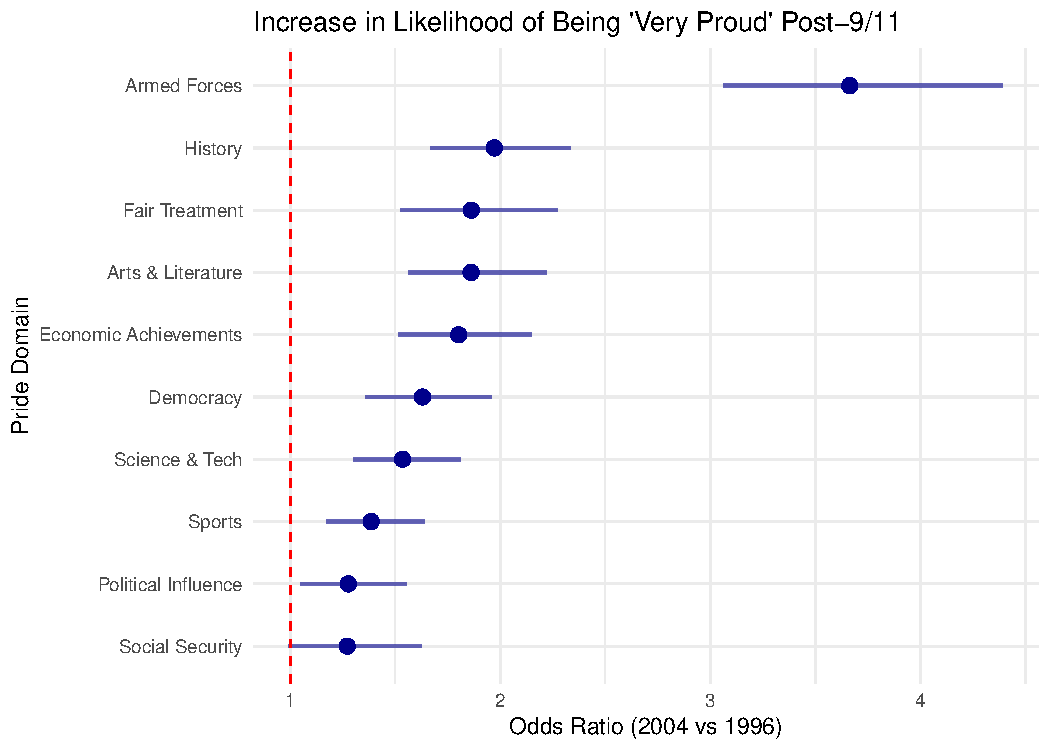
\includegraphics[width=1.0\textwidth]{Plots/fig-logistic-pride.pdf}
\caption{Increase in Likelihood of Being `Very Proud' Post-9/11 (Odds Ratios)}
\label{fig:logistic_pride}
\end{figure}

\begin{figure}[H]
\centering
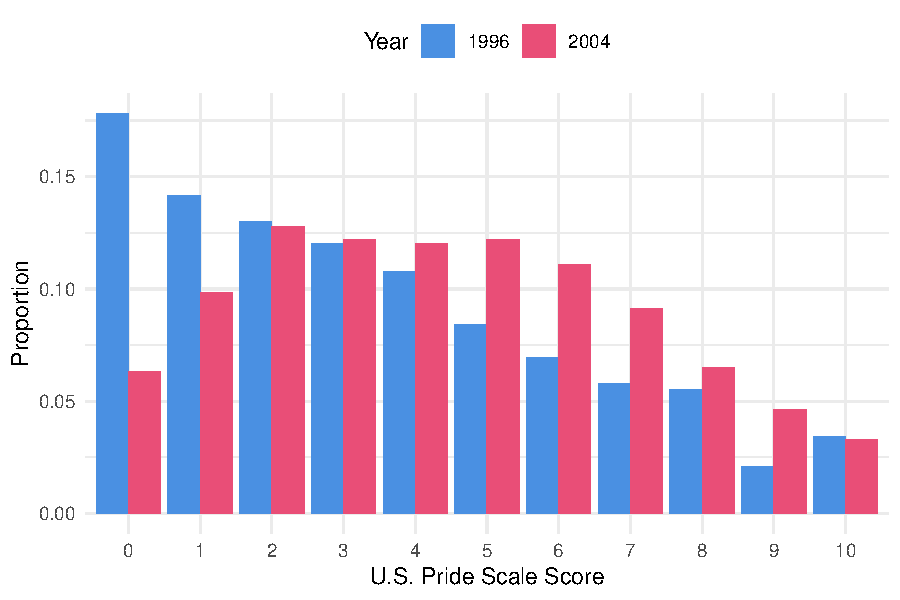
\includegraphics[width=0.8\textwidth]{Plots/fig-pride-bar.pdf}
\caption{Distribution of U.S. Pride Scale Scores (1996 vs. 2004)}
\label{fig:pride_bar}
\end{figure}

\subsection{Nationalism and Irrational Patriotism}

The irrational patriotism perspective predicts that 9/11 should have driven an increase in nationalism, particularly among lower-status and less-educated groups. However, our baseline and interaction models assessing the Nationalism scale yield a different picture. While baseline nationalism was indeed higher among older individuals with lower levels of educational attainment in 1996 \citep{jost2003social-206}, the interaction between education and the survey year on the Nationalism scale is neither statistically nor substantively significant. The need-based and irrational patriotism hypotheses fail to fully capture the changing dynamics of national attachment after 9/11, as the anticipated surge in blindly patriotic nationalism among the dispossessed did not neatly materialize as the primary driver of the 9/11 effect (Table \ref{tab:nationalism}).

\subsection{Education and the Post-9/11 Period Effect}

Turning to the U.S. Pride scale under the Choice-Process framework, we compare the effects of education across the two periods. OLS models reveal a striking reversal. As shown in the first model of Table \ref{tab:educ}, in 1996, education was negatively associated with national pride, supporting the hypothesis that low-status individuals are more likely to feel such pride. However, as we can see in the second model in the same table, the coefficient estimate in 2004 is positive (though not significant at conventional levels). A pooled model that formally tests the interaction between education and the survey year shows a significant positive interaction term, suggesting that national pride increased at a faster rate among higher-educated individuals \textit{after} 9/11. 

This shift directly supports the choice-process prediction: individuals with greater structural autonomy experienced the most dramatic increase in their national attachment patterns under the new distal attribution regime. Figure \ref{fig:marginal_educ} plots the predicted marginal effects of education on the U.S. Pride Scale score, clearly demonstrating the positive slope of education in 2004 in clear contrast to the corresponding negative slope in 1996, opening up a substantial gap between high-education individuals observed in 2004 versus similarly educated individuals observed eight years before. Meanwhile, individuals with low levels of education display similar, statistically indistinguishable, and relatively high levels of national pride in both periods. 

\begin{figure}[H]
\centering
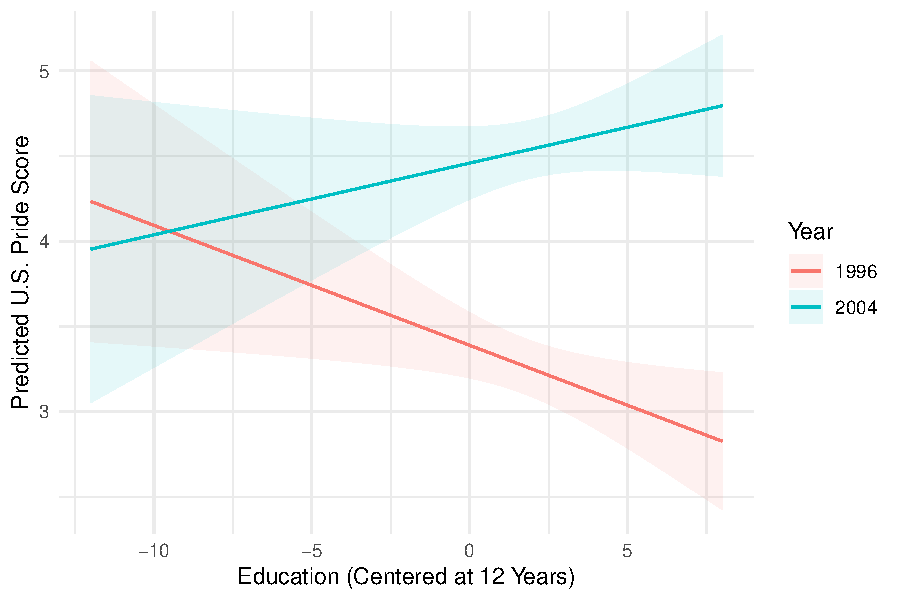
\includegraphics[width=0.8\textwidth]{Plots/fig-marginal-educ.pdf}
\caption{Predicted U.S. Pride Score across Education Levels by Year}
\label{fig:marginal_educ}
\end{figure}

\subsection{Nested Membership and National Attachment}

Following the choice-process framework, we assess how voluntary association membership acts as a nested grouping structure that correlates with attachment to the nation using the 2004 sample. As shown in Table \ref{tab:full2004}, the overall volume of voluntary memberships is a statistically significant, positive predictor of national pride, regardless of whether it is measured as a categorical variable or a continuous count. And this effect is robust to the inclusion of various controls, most notably nationalist sentiment, which is presumably the primary channel through which political ideology (e.g., conservatism) affects feelings of national pride. 

However, a crucial dynamic emerges when disaggregating organizational memberships. According to choice-process theory, affective attachment to the nation requires that the proximate group be cognitively nested within the national structure. Our results confirm this: while the total number of memberships has a positive effect, specific groups that are inherently linked to the national fabric---such as Veterans Groups, Political Clubs, and Fraternal Organizations---foster autonomy that is easily attributed to the larger national collective, resulting in the most substantial increases in U.S. pride. As illustrated in Figure \ref{fig:membership_forest}, these specific nested groups strongly drive the positive relationship between associational embeddedness and national attachment. 

\begin{figure}[H]
\centering
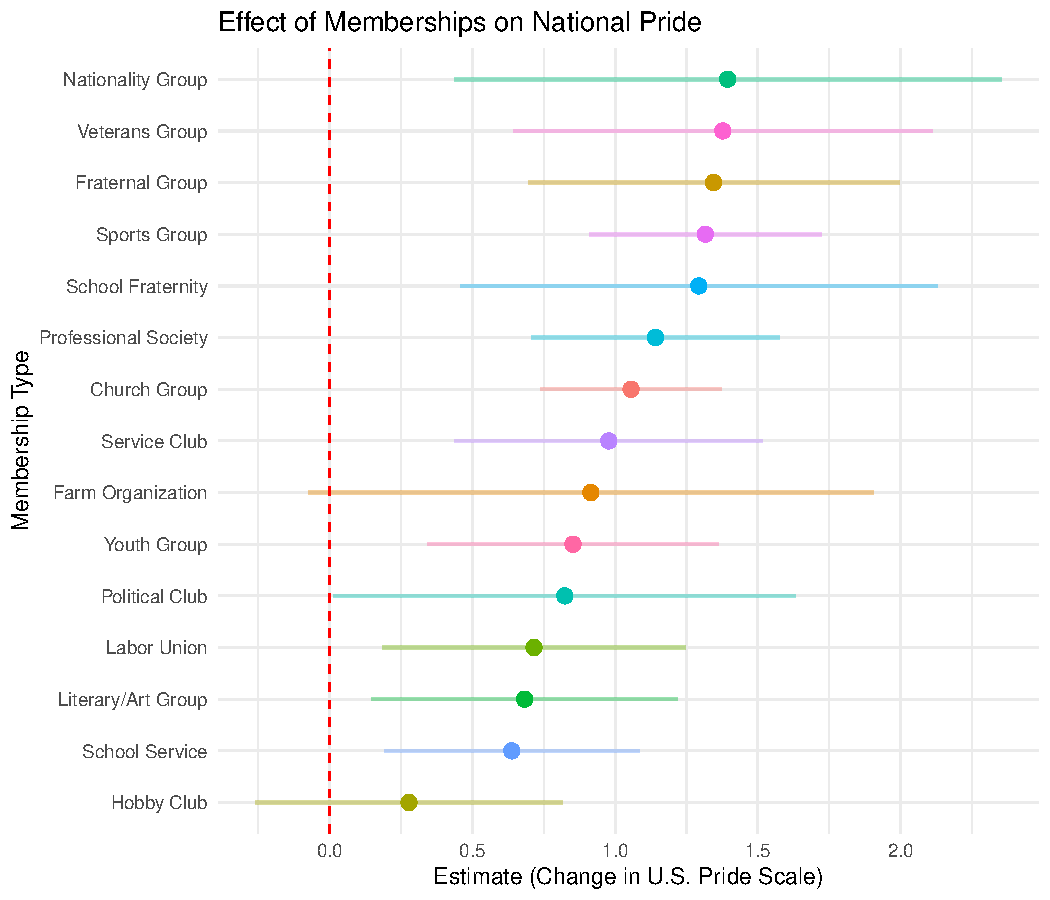
\includegraphics[width=1.0\textwidth]{Plots/fig-membership-forest.pdf}
\caption{Effect of Specific Association Memberships on U.S. Pride (Controlling for Cohort)}
\label{fig:membership_forest}
\end{figure}

\section{Discussion and Conclusion}

\subsection{Summary of Main Results}
This study set out to determine which socio-demographic groups were most likely to experience increased feelings of national pride following a threat to the nation, using the post-9/11 period---catalyzed by the September 11 attacks and encompassing the subsequent wars in Afghanistan and Iraq---as a natural experiment. First, while overall levels of national pride increased significantly across nearly all domains post-9/11, the often-theorized surge in blindly patriotic ``nationalism'' (reflecting a belief in American superiority and uncritical loyalty) was not heavily stratified by socioeconomic status. Although older individuals and those with lower baseline education exhibited higher absolute levels of nationalism, the rate of change in nationalism post-9/11 did not differ significantly by educational attainment.

Second, and in striking contrast, the structural predictors of the affective U.S. Pride scale shifted dramatically. In 1996, education was negatively associated with national pride, aligning with standard expectations that the highly educated display less overt attachment to the nation. However, by 2004, the effect of education on pride had reversed. Highly educated individuals experienced the steepest and most significant increases in national attachment, fundamentally re-ordering the demographic profile of American national pride. 

Third, in the post-9/11 period, embeddedness in voluntary associations proved to be a powerful predictor of this affective attachment. While the total volume of memberships was positively associated with national pride, disaggregating these groups revealed a more specific dynamic. It was specifically embeddedness in groups cognitively linked to the national structure---such as veterans' organizations, political clubs, and fraternal societies---that most powerfully drove the positive relationship between associational life and national pride. 

\subsection{Theoretical Implications}
These findings directly challenge and help to adjudicate between two divergent theoretical perspectives on the nature of national attachment. Standard psychological perspectives on nationalism fall short in predicting \textit{which} individuals were more likely to experience national pride in this new period. Needs-based approaches and theories of ``irrational patriotism'' or authoritarianism predict that those with the most dire needs for belongingness and system justification (typically lower-status, less-educated, and structurally marginalized groups) should experience the most intense increases in their attachment. Our results show that this is definitively not the case. 

Instead, the results are more consistent with Lawler's \citeyearpar{lawler1992affective-8c8} choice-process approach. Over the post-9/11 period, it was precisely those individuals more likely to experience structural autonomy in their day-to-day behavior---the highly educated---who increased their attachment to the national collectivity. In this framework, 9/11 served as the catalyzing event for a sustained, multi-year period of national mobilization---including the invasion of Afghanistan and the Iraq War---across which attribution rules shifted from a ``local'' (proximal) to a ``national'' (distal) orientation. Efficacious action and positive affect generated in structured, local contexts could be attributed to the nation as the ultimate guarantor of those freedoms throughout this period, not only in the immediate wake of the attacks themselves. Furthermore, the strong effect of specific nested groups accounts for exactly how this positive affect generated in local, structured contexts is transferred to the super-ordinate collectivity. 

An important analytical distinction must therefore be maintained between class-based \textit{expression rules} and internal \textit{feeling rules}. While lower-status individuals may have been more likely to \textit{express} national pride in highly visible ways (e.g., via bumper stickers or overt patriotic displays), they were paradoxically less likely as a group to experience a proportional \textit{increase} in affective attachment. High-status individuals embedded in nested groups were actually more likely to \textit{feel} increased national pride after 9/11, even if they were less likely to outwardly express it in stereotypical ways. By shifting our theoretical lens to the choice process, we can better understand the structural and affective foundations of modern patriotism.

\subsection{Limitations and Future Research}
While this study leverages a unique historical juncture to evaluate macro-level shifts in attachment, several limitations in the current effort present opportunities for future research. First, the analysis relies on pooled cross-sectional data from the GSS. Because we observe different, independent samples in 1996 and 2004, we cannot track true within-individual changes in national pride. Future research should engage with longitudinal panel data to observe intra-individual shifts in attribution rules and affective attachments following national crises. Tracking the same individuals would allow researchers to make more robust causal claims about how an individual's pre-crisis structural position conditions their post-crisis emotional response.

Second, data availability constraints prevented the inclusion of political ideology in the primary 2004 models. Although supplementary models on the 1996 subsample demonstrated that the baseline structural effects of education remain robust after adjusting for conservative ideology, and the results in 2004 remain robust to the inclusion of nationalist sentiments (the main mechanism via which political ideology presumably operates), future investigations should leverage datasets in which a more direct adjustment for political ideology is feasible. This would allow researchers to ask novel questions about the independent and interacting roles of political conservatism and structural autonomy over time, exploring whether the choice-process mechanism operates differently across partisan divides. 

Finally, this study relies on educational attainment and voluntary association counts as proxy measures for the structural affordance of autonomy and self-direction. Future studies could address these theoretical mechanisms more directly using different methods. For instance, researchers could directly measure occupational autonomy and subjective self-efficacy via survey instruments, or experimentally manipulate the salience of the distal attribution rule in a laboratory setting. Furthermore, exploring whether other types of national threats---such as economic depressions, severe domestic political polarization, or global pandemics---trigger a similar distal attribution rule, or instead cause a retrenchment into local, proximal attachments, remains an exciting frontier for the sociology of emotions and political sociology.

A related limitation follows directly from our decision to treat 9/11 as the catalyst for a broader post-9/11 period rather than as an isolated, dated stimulus. Because the 2004 GSS wave falls more than two years after the September 11 attacks, the observed shift in national pride cannot be cleanly attributed to 9/11 alone as distinct from the subsequent invasion of Afghanistan, the Iraq War, and the sustained wartime mobilization that followed. We do not view this as a threat to our argument, since the choice-process framework locates the mechanism in the cumulative salience of national rituals and symbols across this period rather than in the September 11 attacks as a single punctual event; the wars are best understood as continuing to supply exactly this kind of salience-raising material rather than as confounds external to the process we theorize. This reframing is consistent with, though it does not fully resolve, the reviewer's observation that the U.S. Pride item for the armed forces in particular is likely shaped by the wars themselves rather than by 9/11 per se. Future work with more temporally granular data---for example, repeated cross-sections spanning 2001--2004---could help disentangle the relative contributions of the initial shock and the subsequent period of wartime mobilization to the overall shift in attribution rules.

\clearpage
\bibliography{references} 

\clearpage
\section*{Tables}

\begin{table}[htbp]
\centering
\caption{Descriptive Statistics for Variables Used in Analysis}
\label{tab:descriptives}
\begin{tabular}{lcccc}
\toprule
\textbf{Continuous Variables} & \textbf{Mean} & \textbf{Std. Dev.} & \textbf{Min} & \textbf{Max} \\
\midrule
U.S. Pride Scale & 3.88 & 2.79 & 0.0 & 10.0 \\
Nationalism Scale & 3.72 & .71 & 1.0 & 5.0 \\
Education (Years) & 13.53 & 2.91 & 0.0 & 20.0 \\
Birth Cohort & 1954.57 & 17.18 & 1907 & 1986 \\
Total Memberships & 1.61 & 1.88 & 0.0 & 13.0 \\
\midrule
\textbf{Categorical Variables} & \textbf{\% Yes} & & & \\
\midrule
Female & 55.1\% & & & \\
Race: White & 80.2\% & & & \\
Race: Black & 13.6\% & & & \\
Race: Other & 6.2\% & & & \\
Region: South & 36.7\% & & & \\
Political Ideology: Conservative & 20.5\% & & & \\
\midrule
\textbf{Voluntary Association Memberships} & \textbf{\% Yes} & & & \\
\midrule
Church-affiliated & 31.0\% & & & \\
Sports & 16.8\% & & & \\
Professional & 15.1\% & & & \\
School & 14.1\% & & & \\
Hobby & 10.8\% & & & \\
Literary or Art & 10.5\% & & & \\
Youth & 10.3\% & & & \\
Labor Union & 9.6\% & & & \\
Service & 9.6\% & & & \\
Fraternal & 6.8\% & & & \\
Veterans & 5.3\% & & & \\
Political & 4.3\% & & & \\
School Fraternity/Sorority & 4.2\% & & & \\
Farm & 3.0\% & & & \\
Nationality & 2.7\% & & & \\
\bottomrule
\end{tabular}
\end{table}

\clearpage
\begin{table}
\centering
\begin{talltblr}[         %% tabularray outer open
caption={Predictors of Nationalism Scale (1996 vs 2004)},
label={tab:nationalism},
note{}={Note: + p \num{< .1}, * p \num{< .05}, ** p \num{< .01}, *** p \num{< .001}},
]                     %% tabularray outer close
{                     %% tabularray inner open
colspec={Q[]Q[]Q[]},
hline{2}={1-3}{solid, black, .05em},
hline{12}={1-3}{solid, black, .05em},
hline{1}={1-3}{solid, black, .08em},
hline{20}={1-3}{solid, black, .08em},
column{2-3}={}{halign=c},
column{1}={}{halign=l},
}                     %% tabularray inner close
& Base Change & Educ Interaction \\
Education (Years) &  & \num{-.053}*** \\
&  & (\num{.007}) \\
Birth Cohort & \num{-.010}*** & \num{-.009}*** \\
& (\num{.001}) & (\num{.001}) \\
Year: 2004 & \num{.134}*** & \num{.190} \\
& (\num{.028}) & (\num{.135}) \\
Education × Year 2004 &  & \num{-.003} \\
&  & (\num{.010}) \\
Intercept & \num{22.352}*** & \num{21.858}*** \\
& (\num{1.645}) & (\num{1.607}) \\
Num.Obs. & \num{2558} & \num{2555} \\
R2 & \num{.050} & \num{.096} \\
R2 Adj. & \num{.049} & \num{.094} \\
AIC & \num{5630.1} & \num{5500.9} \\
BIC & \num{5653.5} & \num{5535.9} \\
Log.Lik. & \num{-2811.070} & \num{-2744.434} \\
F & \num{67.404} & \num{67.571} \\
RMSE & \num{.70} & \num{.67} \\
\end{talltblr}
\end{table}


\clearpage
\begin{table}
\centering
\begin{talltblr}[         %% tabularray outer open
caption={Effects of Education on U.S. Pride Scale (1996 vs 2004)},
label={tab:educ},
note{}={Note: + p \num{< .1}, * p \num{< .05}, ** p \num{< .01}, *** p \num{< .001}},
]                     %% tabularray outer close
{                     %% tabularray inner open
colspec={Q[]Q[]Q[]Q[]},
hline{2}={1-4}{solid, black, .05em},
hline{12}={1-4}{solid, black, .05em},
hline{1}={1-4}{solid, black, .08em},
hline{19}={1-4}{solid, black, .08em},
column{2-4}={}{halign=c},
column{1}={}{halign=l},
}                     %% tabularray inner close
& 1996 & 2004 & Pooled Interaction \\
Education (Years) & \num{-.066}* & \num{.040} & \num{-.072}* \\
& (\num{.030}) & (\num{.032}) & (\num{.030}) \\
Birth Cohort & \num{-.047}*** & \num{-.028}*** & \num{-.038}*** \\
& (\num{.005}) & (\num{.005}) & (\num{.004}) \\
Year: 2004 &  &  & \num{-.343} \\
&  &  & (\num{.624}) \\
Education × Year 2004 &  &  & \num{.114}** \\
&  &  & (\num{.044}) \\
Intercept & \num{96.569}*** & \num{59.411}*** & \num{79.100}*** \\
& (\num{10.017}) & (\num{10.314}) & (\num{7.183}) \\
Num.Obs. & \num{1066} & \num{975} & \num{2041} \\
R2 & \num{.081} & \num{.030} & \num{.084} \\
R2 Adj. & \num{.080} & \num{.028} & \num{.083} \\
AIC & \num{5239.6} & \num{4778.3} & \num{10021.1} \\
BIC & \num{5259.4} & \num{4797.8} & \num{10054.8} \\
Log.Lik. & \num{-2615.781} & \num{-2385.153} & \num{-5004.531} \\
RMSE & \num{2.73} & \num{2.60} & \num{2.67} \\
\end{talltblr}
\end{table}


\clearpage
\begin{table}
\centering
\begin{talltblr}[         %% tabularray outer open
caption={Predictors of U.S. Pride (2004 sample only)},
label={tab:full2004},
note{}={Note: + p \num{< .1}, * p \num{< .05}, ** p \num{< .01}, *** p \num{< .001}},
]                     %% tabularray outer close
{                     %% tabularray inner open
colspec={Q[]Q[]Q[]Q[]Q[]},
hline{2}={1-5}{solid, black, .05em},
hline{24}={1-5}{solid, black, .05em},
hline{1}={1-5}{solid, black, .08em},
hline{31}={1-5}{solid, black, .08em},
column{2-5}={}{halign=c},
column{1}={}{halign=l},
}                     %% tabularray inner close
& Demographics & Mem (Cat) & Mem (Count) & Full (+ Nat) \\
Education (Years) & \num{.017} & \num{-.010} & \num{-.007} & \num{.059}+ \\
& (\num{.032}) & (\num{.033}) & (\num{.033}) & (\num{.032}) \\
Birth Cohort & \num{-.025}*** & \num{-.024}*** & \num{-.024}*** & \num{-.016}** \\
& (\num{.005}) & (\num{.005}) & (\num{.005}) & (\num{.005}) \\
Female & \num{-.706}*** & \num{-.677}*** & \num{-.679}*** & \num{-.583}*** \\
& (\num{.167}) & (\num{.167}) & (\num{.167}) & (\num{.160}) \\
Race: Black & \num{-1.331}*** & \num{-1.355}*** & \num{-1.373}*** & \num{-1.165}*** \\
& (\num{.260}) & (\num{.260}) & (\num{.261}) & (\num{.250}) \\
Race: Other & \num{-.087} & \num{-.036} & \num{-.060} & \num{-.064} \\
& (\num{.339}) & (\num{.339}) & (\num{.339}) & (\num{.324}) \\
Region: South & \num{.256} & \num{.250} & \num{.252} & \num{.146} \\
& (\num{.177}) & (\num{.177}) & (\num{.177}) & (\num{.170}) \\
Nationalist Scale &  &  &  & \num{1.164}*** \\
&  &  &  & (\num{.122}) \\
Total Memberships (Count) &  &  & \num{.115}* & \num{.112}** \\
&  &  & (\num{.045}) & (\num{.043}) \\
Memberships: 1-2 &  & \num{.406}* &  &  \\
&  & (\num{.199}) &  &  \\
Memberships: 3+ &  & \num{.680}** &  &  \\
&  & (\num{.221}) &  &  \\
Intercept & \num{53.833}*** & \num{51.190}*** & \num{51.826}*** & \num{31.206}** \\
& (\num{10.188}) & (\num{10.200}) & (\num{10.204}) & (\num{9.992}) \\
Num.Obs. & \num{975} & \num{974} & \num{974} & \num{974} \\
R2 & \num{.071} & \num{.081} & \num{.077} & \num{.157} \\
R2 Adj. & \num{.066} & \num{.073} & \num{.071} & \num{.150} \\
AIC & \num{4743.7} & \num{4735.3} & \num{4736.6} & \num{4650.3} \\
BIC & \num{4782.8} & \num{4784.1} & \num{4780.5} & \num{4699.1} \\
Log.Lik. & \num{-2363.873} & \num{-2357.626} & \num{-2359.299} & \num{-2315.136} \\
RMSE & \num{2.56} & \num{2.55} & \num{2.55} & \num{2.41} \\
\end{talltblr}
\end{table}


\newpage
\appendix
\section{Supplementary Models with Political Ideology (1996 Only)}

Because the 2004 GSS administered the political ideology and national attachment modules on mutually exclusive survey ballots, it is impossible to adjust for political ideology in pooled models or models using the 2004 sample. However, given the theoretical relevance of conservative political ideology to national attachment, we present our core models predicting the Nationalism and U.S. Pride scales here restricted to the 1996 subsample of respondents who provided valid responses for both political ideology and the dependent variables.

\newpage
\begin{table}
\centering
\begin{talltblr}[         %% tabularray outer open
caption={Predictors of Nationalism Scale (1996 Subsample with Ideology)},
note{}={Note: + p \num{< .1}, * p \num{< .05}, ** p \num{< .01}, *** p \num{< .001}},
]                     %% tabularray outer close
{                     %% tabularray inner open
colspec={Q[]Q[]Q[]},
hline{2}={1-3}{solid, black, .05em},
hline{10}={1-3}{solid, black, .05em},
hline{1}={1-3}{solid, black, .08em},
hline{18}={1-3}{solid, black, .08em},
column{2-3}={}{halign=c},
column{1}={}{halign=l},
}                     %% tabularray inner close
& Base Change & With Educ \\
Education (Years) &  & \num{-.053}*** \\
&  & (\num{.007}) \\
Birth Cohort & \num{-.010}*** & \num{-.009}*** \\
& (\num{.001}) & (\num{.001}) \\
Political Ideology (Conservative) & \num{.178}*** & \num{.196}*** \\
& (\num{.048}) & (\num{.047}) \\
Intercept & \num{23.425}*** & \num{22.082}*** \\
& (\num{2.279}) & (\num{2.237}) \\
Num.Obs. & \num{1281} & \num{1279} \\
R2 & \num{.069} & \num{.113} \\
R2 Adj. & \num{.068} & \num{.111} \\
AIC & \num{2750.2} & \num{2687.3} \\
BIC & \num{2770.8} & \num{2713.0} \\
Log.Lik. & \num{-1371.109} & \num{-1338.640} \\
F & \num{47.653} &  \\
RMSE & \num{.68} & \num{.66} \\
\end{talltblr}
\end{table}


\clearpage
\begin{table}
\centering
\begin{talltblr}[         %% tabularray outer open
caption={Effects of Education on U.S. Pride Scale (1996 Subsample with Ideology)},
note{}={Note: + p \num{< .1}, * p \num{< .05}, ** p \num{< .01}, *** p \num{< .001}},
]                     %% tabularray outer close
{                     %% tabularray inner open
colspec={Q[]Q[]},
hline{2}={1-2}{solid, black, .05em},
hline{10}={1-2}{solid, black, .05em},
hline{1}={1-2}{solid, black, .08em},
hline{17}={1-2}{solid, black, .08em},
column{2}={}{halign=c},
column{1}={}{halign=l},
}                     %% tabularray inner close
& 1996 \\
Education (Years) & \num{-.063}* \\
& (\num{.031}) \\
Birth Cohort & \num{-.046}*** \\
& (\num{.005}) \\
Political Ideology (Conservative) & \num{.687}*** \\
& (\num{.207}) \\
Intercept & \num{94.622}*** \\
& (\num{10.124}) \\
Num.Obs. & \num{1029} \\
R2 & \num{.094} \\
R2 Adj. & \num{.092} \\
AIC & \num{5033.7} \\
BIC & \num{5058.4} \\
Log.Lik. & \num{-2511.842} \\
RMSE & \num{2.70} \\
\end{talltblr}
\end{table}


\end{document}